\begin{frame}{Ilustração do impacto da modulação}
	Com a possibilidade da modulação de carga, é possível verificar o impacto da carga modulada no ambiente projetado para o trabalho de \cite{Edwin2015}.
\end{frame}
	
\begin{frame}{Ambiente Computacional do experimento}
	\begin{columns}
		\column{0.4\textwidth}
		\begin{minipage}[c][0.4\textheight][c]{\linewidth}
			\centering
			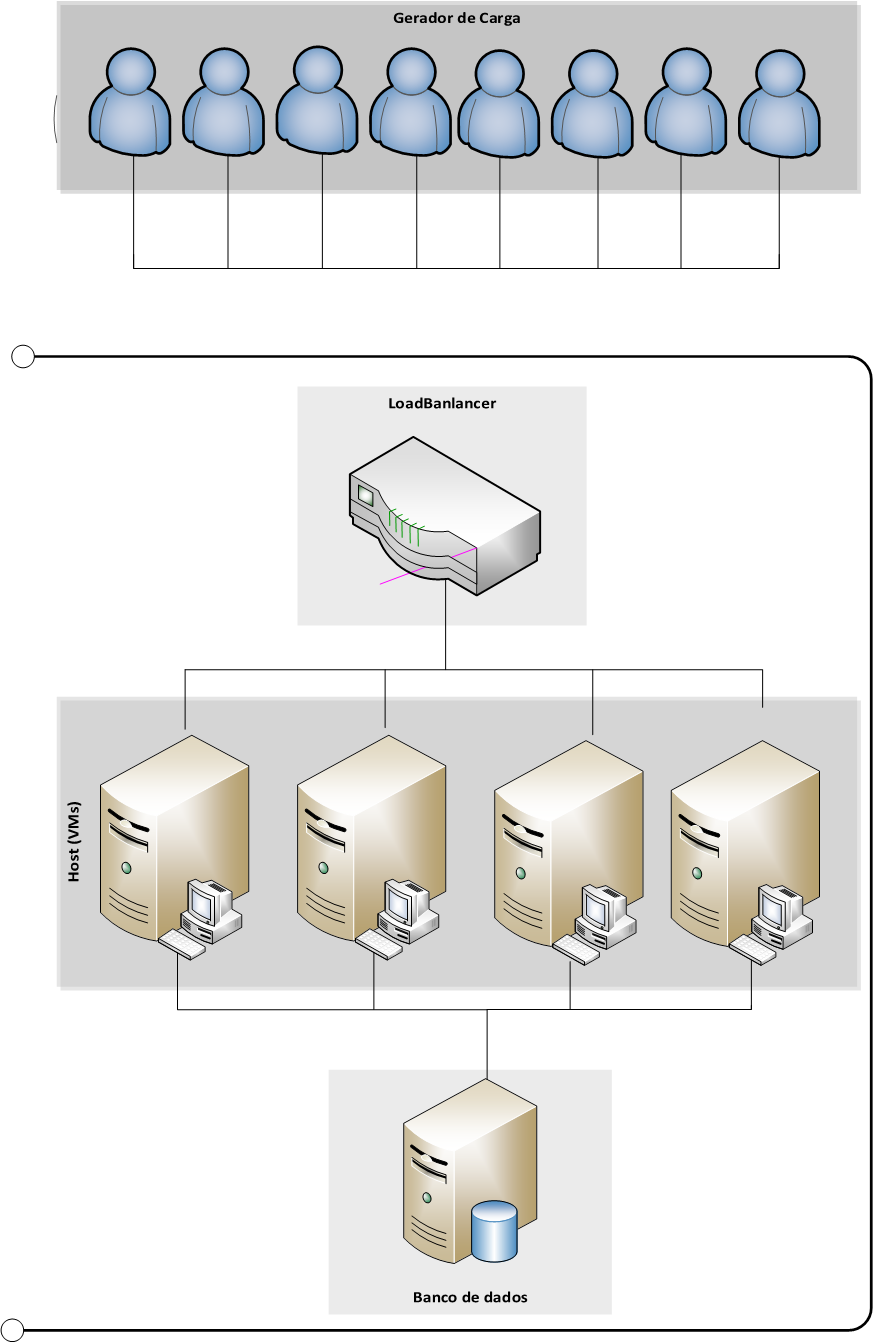
\includegraphics[scale=0.17]{../monograph/images/arquitetura-experimento.png}		
		\end{minipage}
		\column{0.6\textwidth}
		\begin{minipage}[c][0.4\textheight][c]{\linewidth}
			\begin{itemize}
				\item Gerador de Carga (\textit{Workload})
				\item Balanceador de carga (\textit{Load Balancer})
				\item Servidor Físico (\textit{Hypervisor})
				\item Servidor de dados (\textit{Data base})
			\end{itemize}
			\begin{figure}
				\centering
				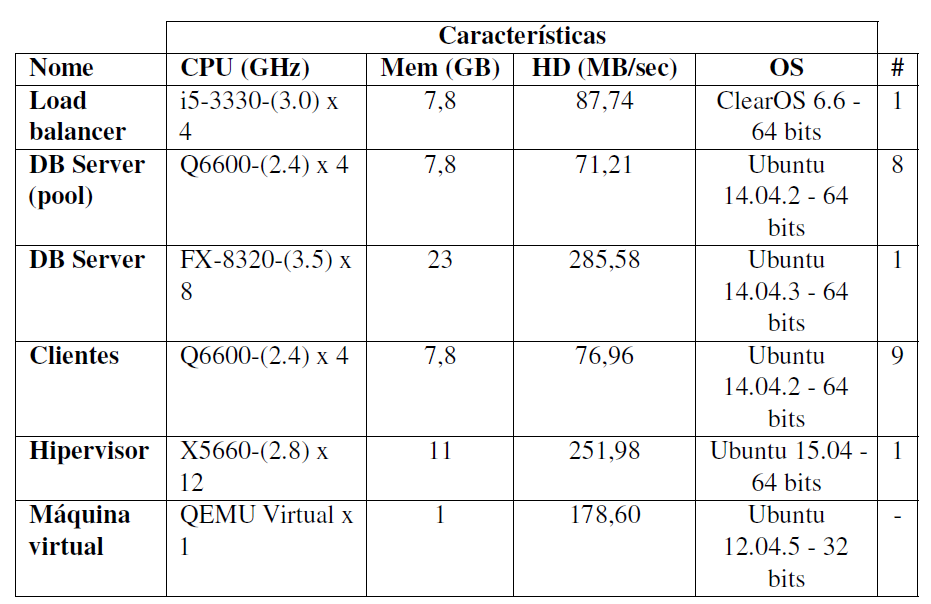
\includegraphics[scale=0.25]{images/soft-hard.png}
			\end{figure}
		\end{minipage}		
	\end{columns}
	
\end{frame}

%\begin{frame}{Elementos utilizados nos experimentos}
%	\begin{itemize}
%		\item Instalações do LaSDPC;
%		\item Foram utilizados dois \textit{clusters}.
%	\end{itemize}
%	\begin{figure}
%		\centering
%		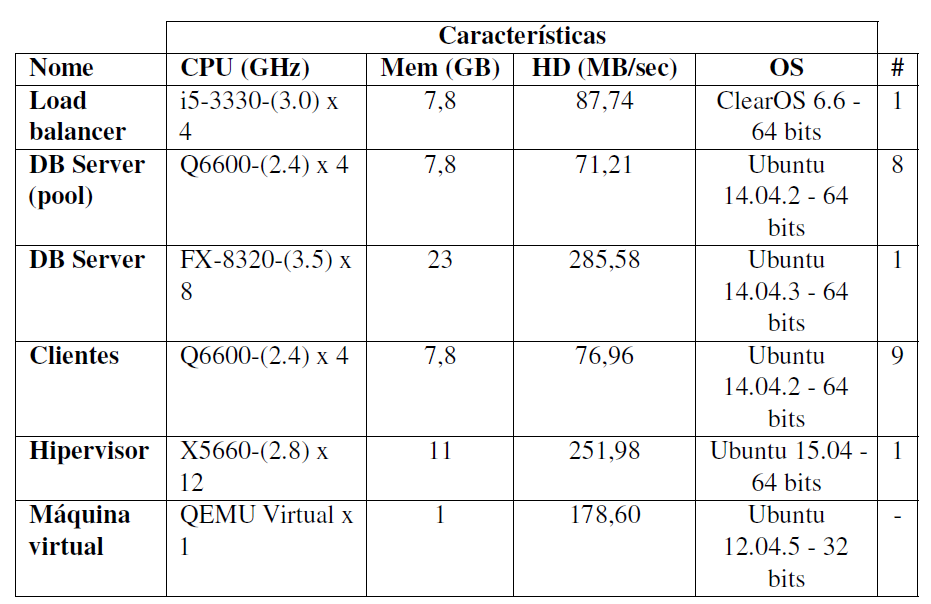
\includegraphics[width=0.6\textwidth]{images/soft-hard.png}
%		\caption{\textit{Hardware} e \textit{software} utilizados nos experimentos.}
%		\label{fig:table}
%	\end{figure}
%\end{frame}

\begin{frame}{Planejamento do experimento}
	\begin{columns}
		\column{0.5\textwidth}
		\begin{minipage}[c][0.4\textheight][c]{\linewidth}
			\centering
			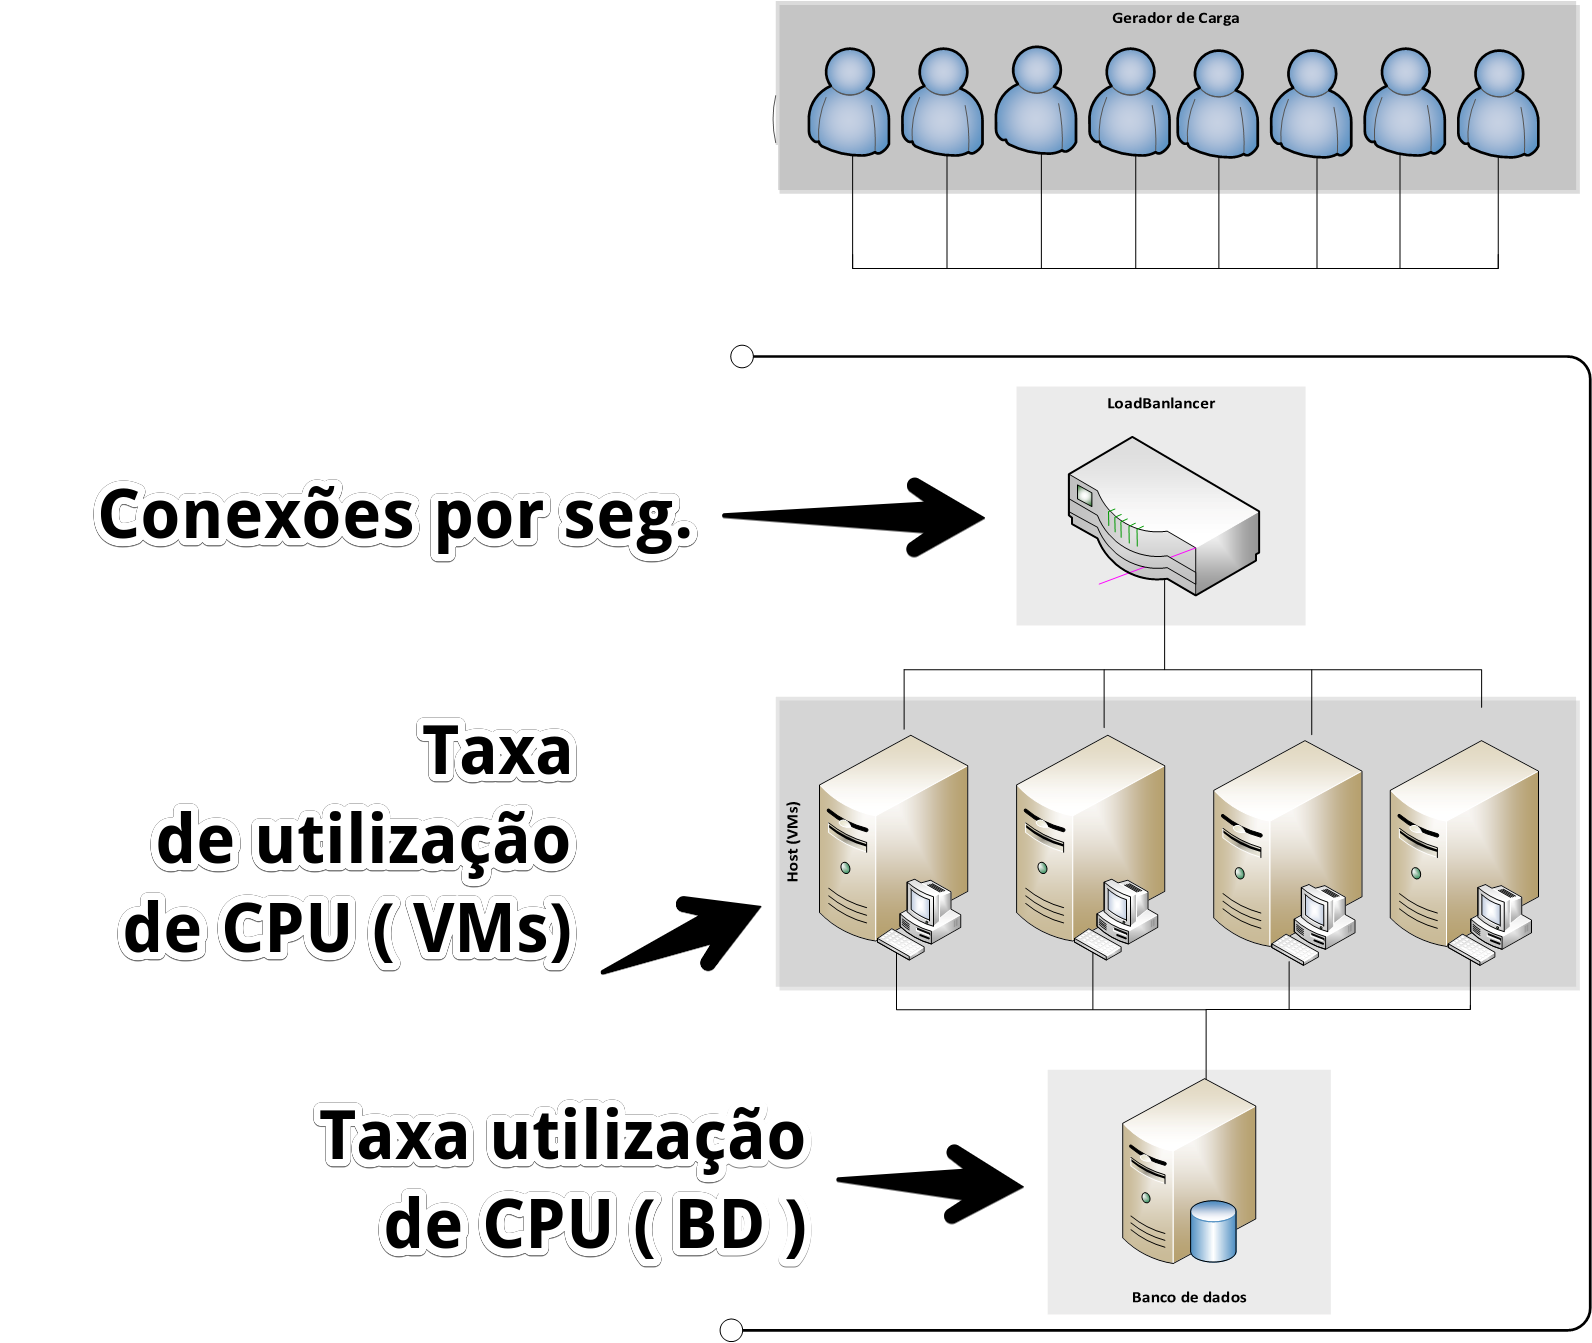
\includegraphics[scale=0.15]{images/metricas-arquitetura-experimento2.png}		
		\end{minipage}
		\column{0.5\textwidth}
		\begin{minipage}[c][0.4\textheight][c]{\linewidth}
			\begin{itemize}
				\item Carga inicial: (10 EBs)
				\item Carga reservada: (20 EBs)
			\end{itemize}
			\begin{figure}
				\centering
				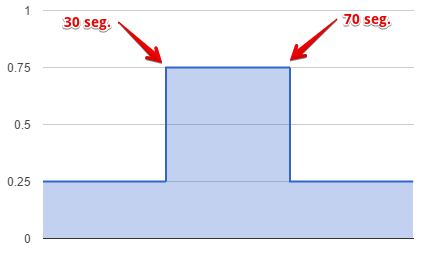
\includegraphics[scale=0.5]{images/carga-modulada-experimento.png}
			\end{figure}
			
		\end{minipage}		
	\end{columns}
	
\end{frame}

%\begin{frame}{Métrica transiente}
%	\begin{itemize}
%		\item \textbf{Conexões por segundo (\textit{Load Balancer}):} Conforme sugerido por \cite{Binnig2009}, medir a escalabilidade através do aumento dos interações web emitidos por segundo ao longo do tempo e de forma contínua contando a interação web que são respondidas em um intervalo de tempo de resposta,
%		
%		\item \textbf{Tempo de resposta (\textit{browsers}):} \cite{helder2014}, em um sistema dinâmico, cuja transformação entrada-saída não ocorre em tempo zero, mas é sujeita a uma inércia advinda dos processos físicos associados, possuí uma inércia intrínseca que atrasa o efeito que uma entrada terá na saída. Esses efeitos refletem no consequentemente nos comportamentos diversos que incluem retardo no tempo de resposta e possíveis oscilações; 	
%		
%	\end{itemize}
%\end{frame}
%
%\begin{frame}{Métrica transiente}
%	\begin{itemize}
%		\item \textbf{Taxa de utilização da CPU (VMs):} \cite{Nobile2013} afirma que diversas métricas podem ser analisadas para verificar o desempenho das máquinas virtuais, e cita alguns exemplos, como o tempo de inicialização, a taxa de utilização de CPU, o tempo médio de resposta e o \textit{throughput}, e usualmente, número de máquinas virtuais que hospedam serviços de interesse ao cliente e que respondem a uma carga de trabalho imposta por usuários através de requisições;
%		
%		\item \textbf{Taxa de utilização da CPU:} O trabalho apresentado por \cite{wang2009}, que lida com uma carga de trabalho variante no tempo e intensiva, demonstra que a CPU e I/O podem ser utilizadas para prever as necessidades dos recursos de um banco de dados e para orientar a alocação de recursos \textit{on-demand} de acordo com a exigência de carga de trabalho. Entretanto iremos somente considerar em nossos experimento a taxa de utilização do banco de dados.
%	\end{itemize}
%\end{frame}

%\begin{frame}{Resultados experimento}
%Com a possibilidade da modulação de carga, é possível verificar o impacto da carga modulada no ambiente projetado para o trabalho de \cite{Edwin2015}. 
%	\begin{itemize}
%		\item inicialmente utilizado 40\% da carga até o instante de 30 segundos de experimentação
%	
%		\item a partir de 30 segundos um crescimento brusco na carga utilizando os 60\% restante da carga, e gerando um degrau positivo. A carga mantém-se máxima, em 100\%, durante 40 segundos 
%	
%		\item apos decorridos 70 segundo de experimentação), a uma queda súbita voltando a trabalhar com 40\% da carga até o final do experimento.
%	\end{itemize}
%\end{frame}

%\begin{frame}{Conexões por segundo vs Tempo de resposta}
%	\begin{figure}[htb]
%		\centering
%		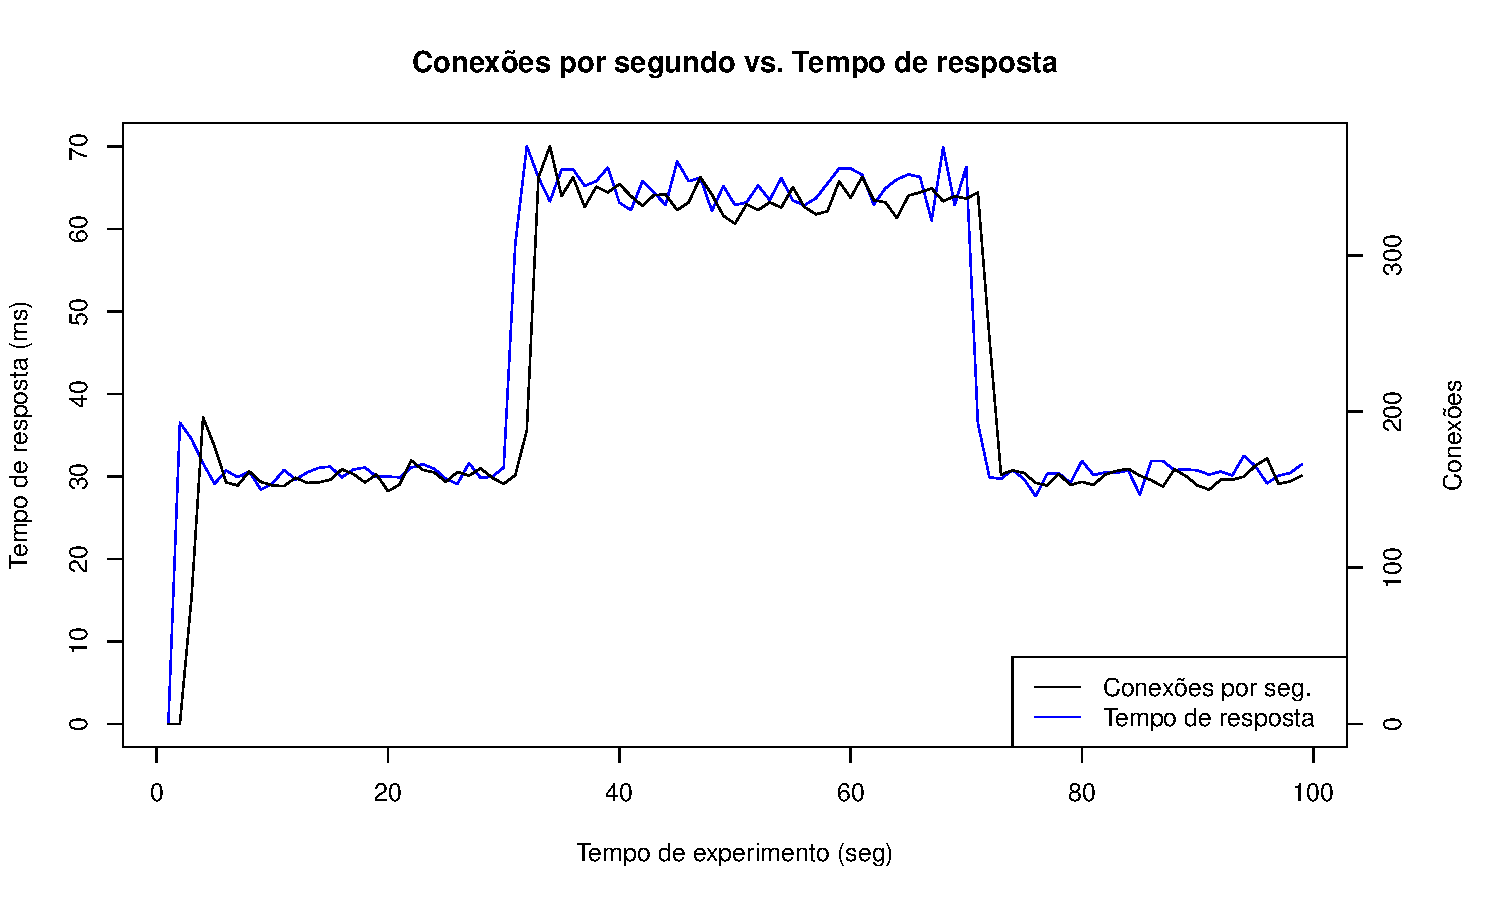
\includegraphics[scale=0.5]{../monograph/images/cps-resp60.pdf}	
%		\label{fig:cps-resp60}
%	\end{figure}
%\end{frame}

\begin{frame}{Conexões por segundo \& Média de utilização das CPU VMs}
	\begin{figure}[htb]
		\centering
		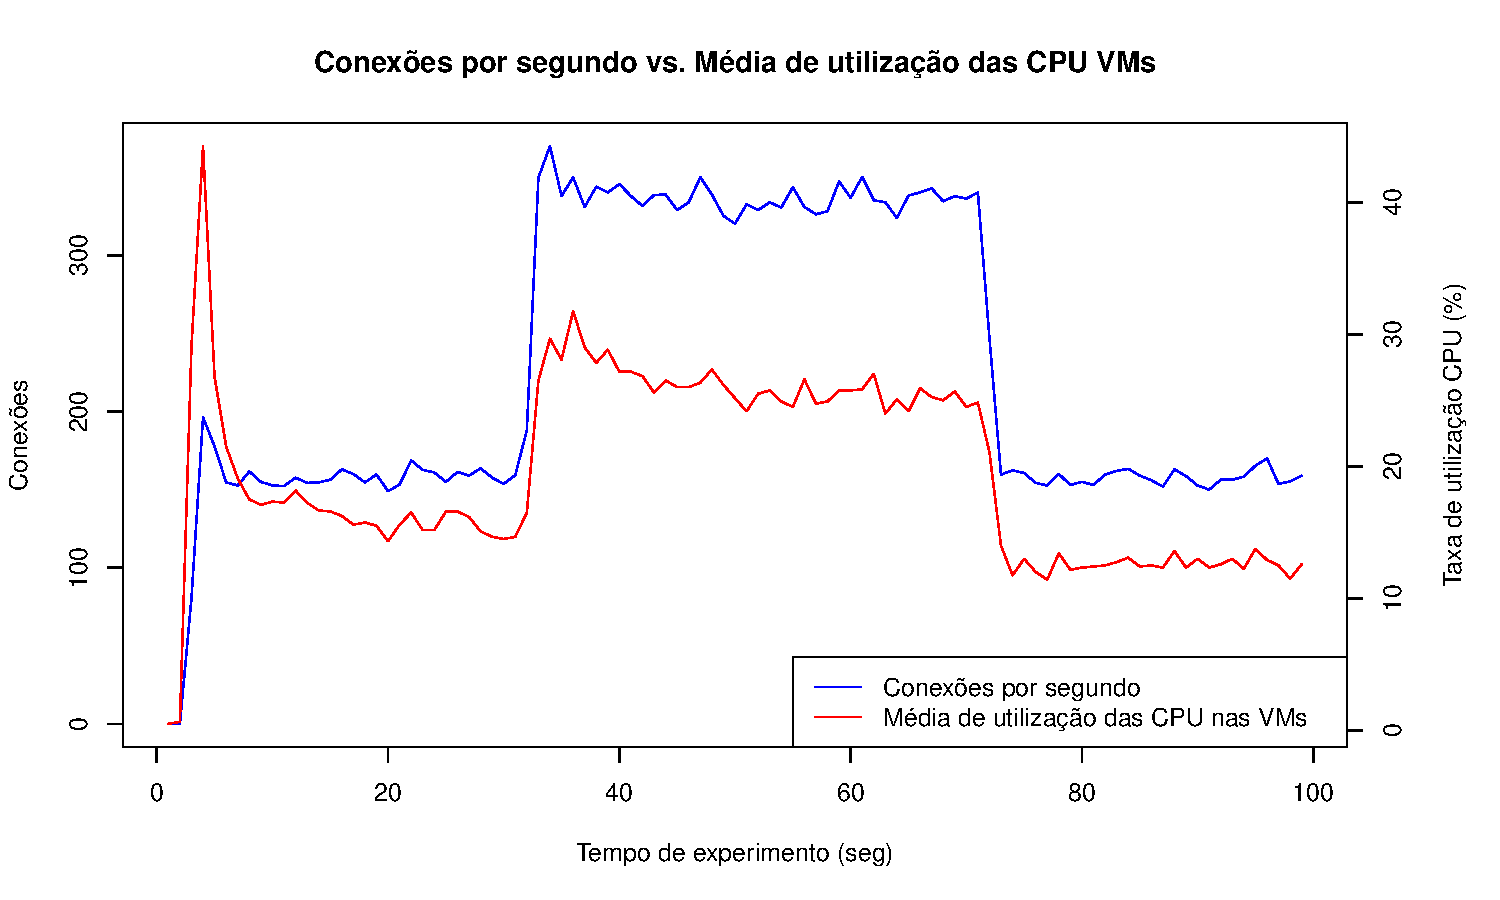
\includegraphics[scale=0.45]{../monograph/images/cps-vmcpu60.pdf}
		\label{fig:cps-vmcpu60}
	\end{figure}
\end{frame}

\begin{frame}{Conexões por segundo \& Utilização de CPU Banco de dados}
	\begin{figure}[htb]
		\centering
		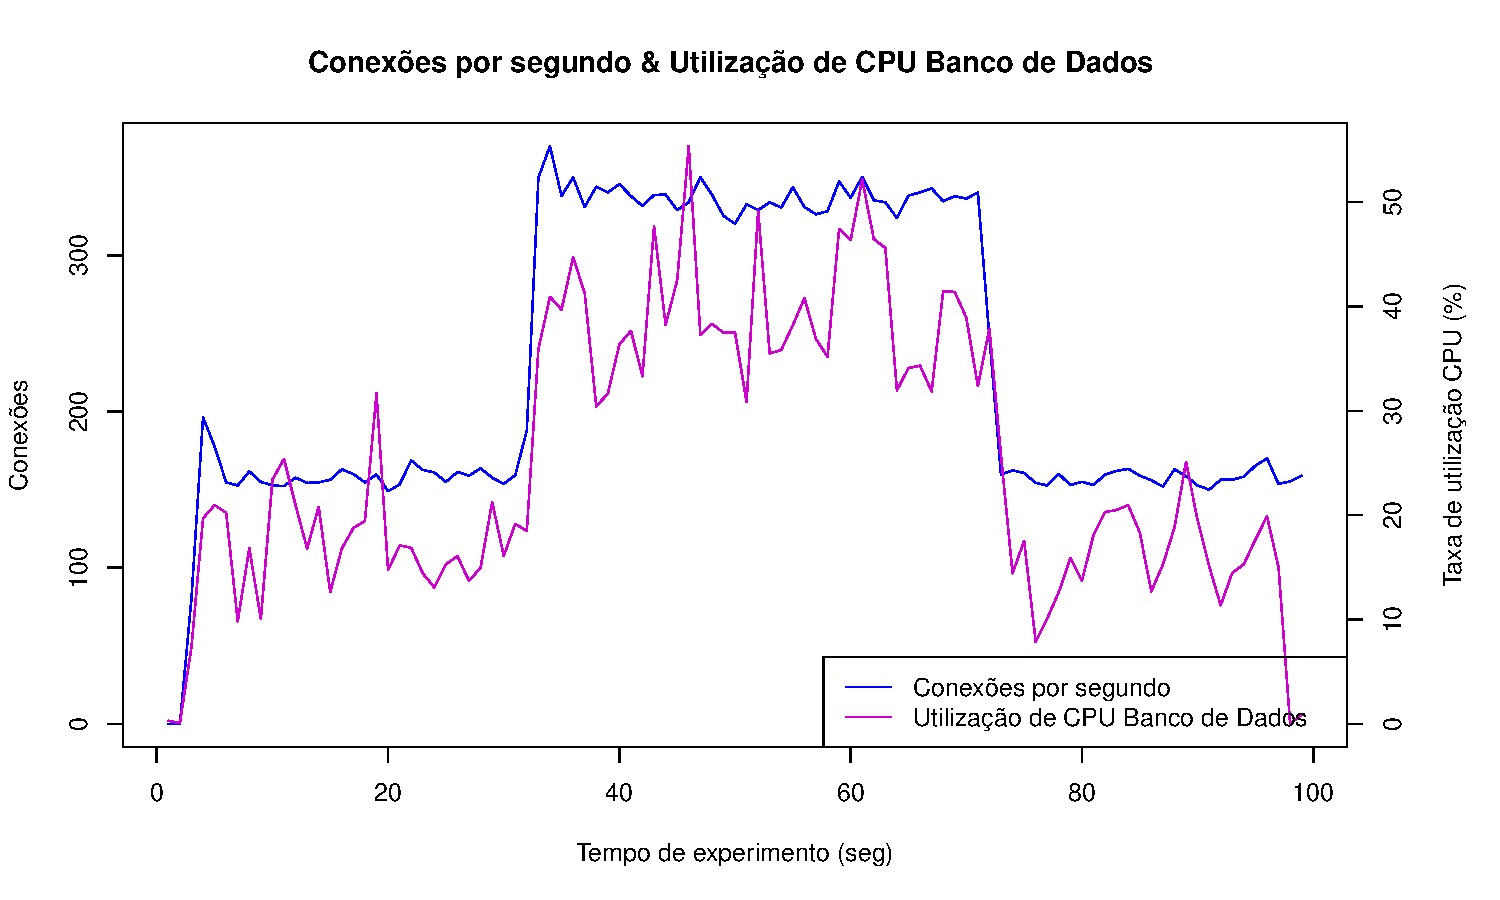
\includegraphics[scale=0.45]{../monograph/images/cps-dbcpu60.pdf}
		\label{fig:cps-dbcpu60}
	\end{figure}
\end{frame}

%\begin{frame}{Tempo de resposta \& Utilização de CPU Banco de dados}
%	\begin{figure}[htb]
%		\centering
%		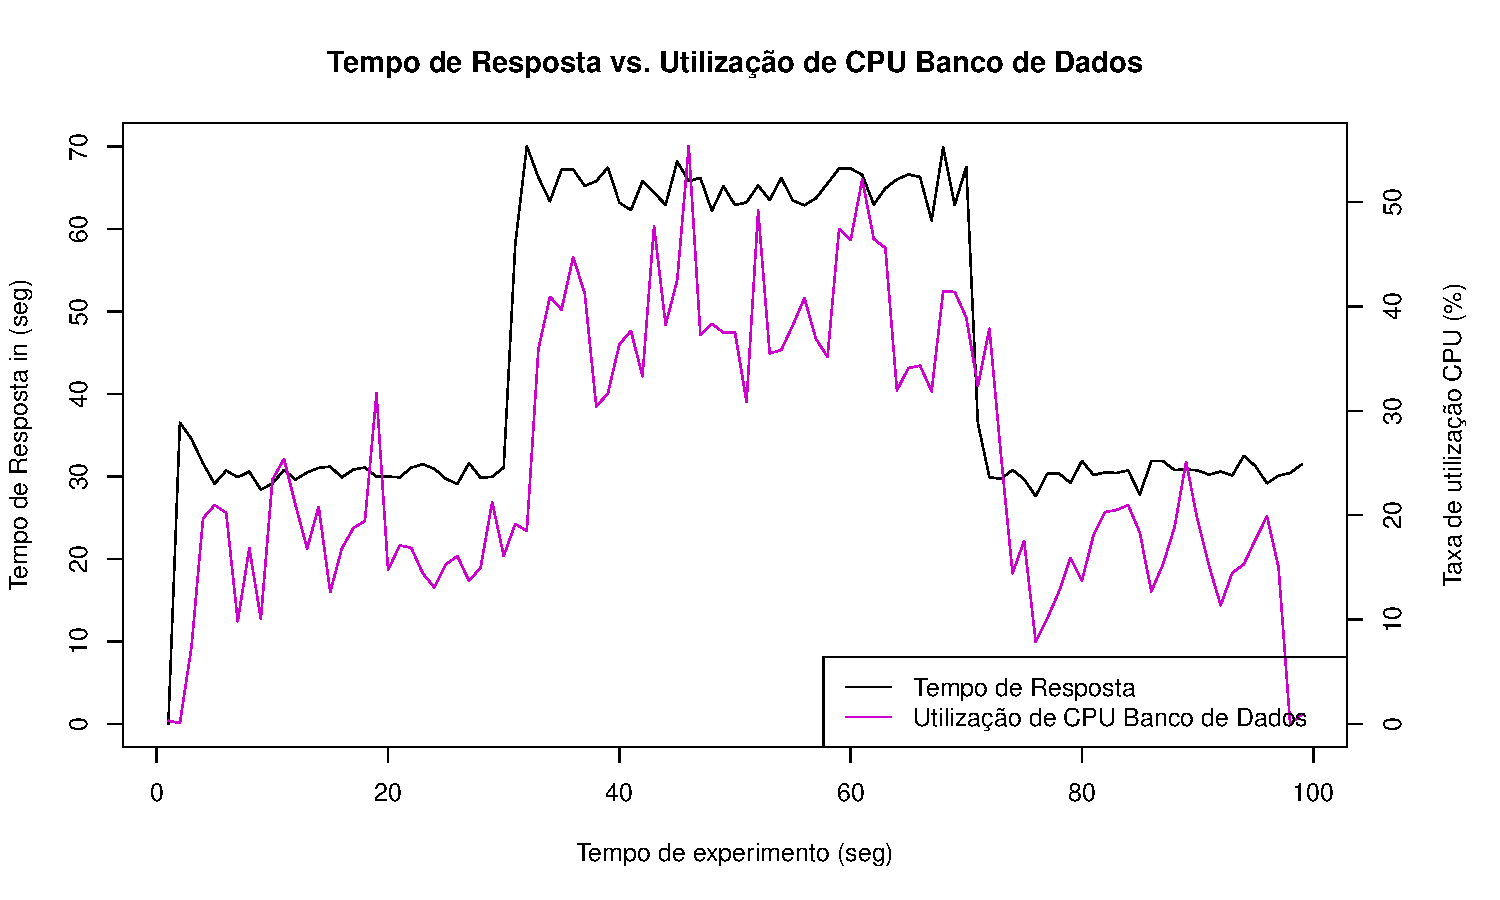
\includegraphics[scale=0.45]{../monograph/images/resp-dbcpu60.pdf}
%		\label{fig:resp-dbcpu60}
%	\end{figure}
%\end{frame}

\begin{frame}{Comparação PostgreSQL e DB2}
	\begin{columns}
		\begin{column}{0.5\textwidth}
			\begin{figure}
				\centering
				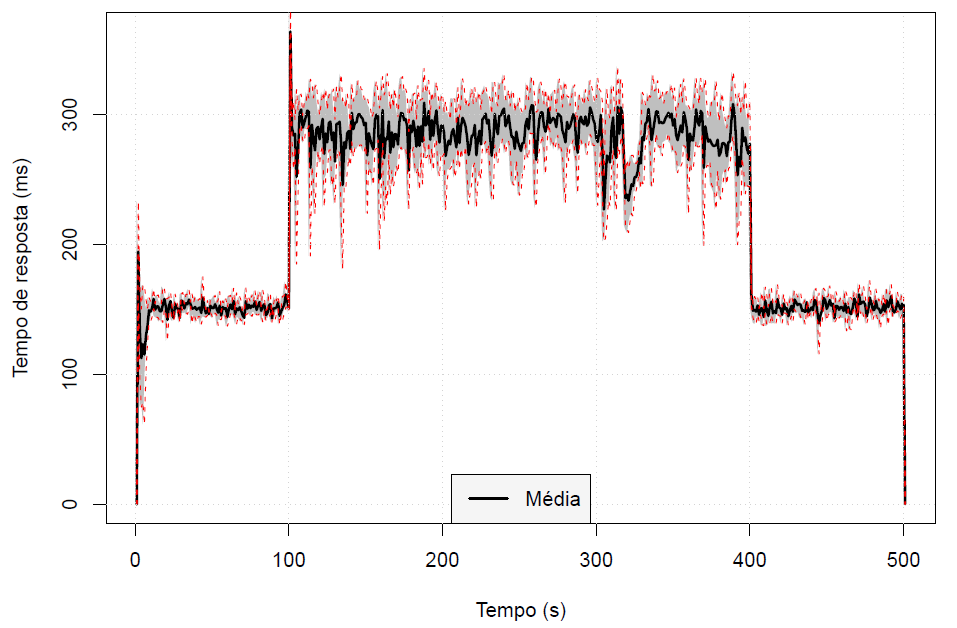
\includegraphics[width=0.9\textwidth]{images/tempo-resposta-postgres-crop.png}
			\end{figure}
			
		\end{column}
		
		\begin{column}{0.5\textwidth}
				\begin{figure}
					\centering
					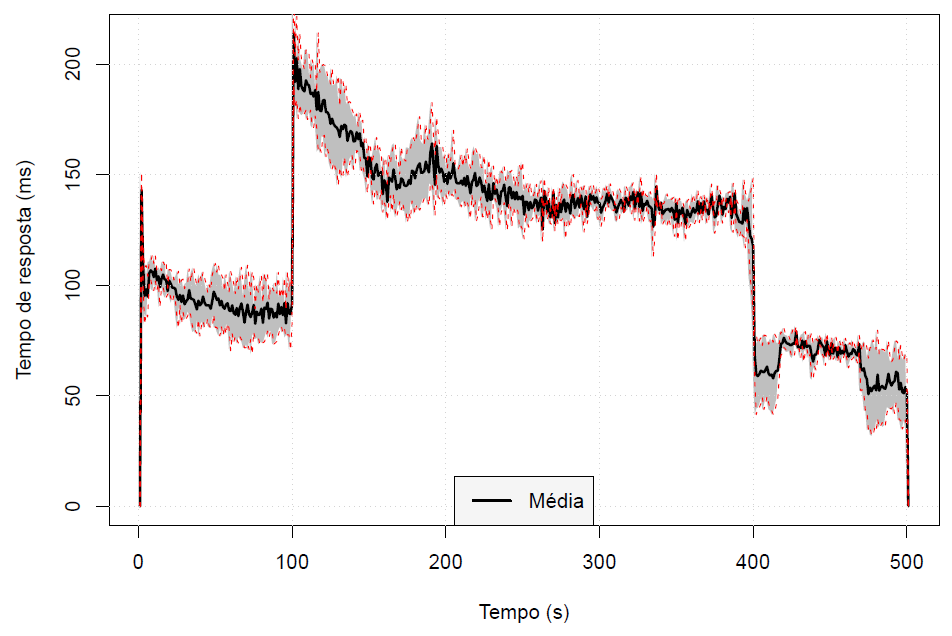
\includegraphics[width=0.9\textwidth]{images/tempo-resposta-db2-crop.png}
				\end{figure}
			
		\end{column}
	\end{columns}
	
	\caption{Resultados trabalho \cite{Edwin2015}}
\end{frame}


\begin{frame}{Utilização da metodologia de avaliação de desempenho não-estacionário}
	\begin{columns}
		\column{0.6\textwidth}
		\begin{figure}[htb]
			\centering
			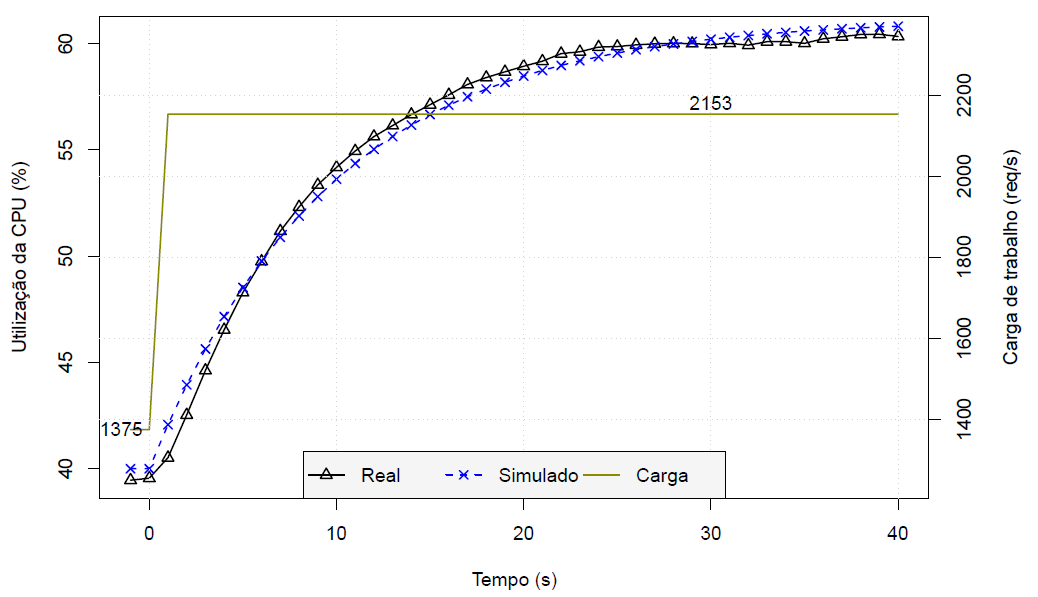
\includegraphics[scale=0.25]{images/resultado_edwin_identificao_sys.png}				
		\end{figure}
		\column{0.4\textwidth}
		\begin{block}{Domínio na frequência}
			\begin{equation}
				\small
				G(z) = \frac{b}{z - a}
			\end{equation}			
			\begin{equation}
				\small
				G(z) = \frac{0.002682}{z - 0.9057}
			\end{equation}							
		\end{block}
		\caption{Resultados trabalho \cite{Edwin2015}}				
				
	\end{columns}
	\begin{block}{Domínio no tempo}
		\begin{equation}
			\small	
			y(k) = -ay(k-1) + bu(k-1)
		\end{equation}			
		\begin{equation}
			\small
			y(k) = -0.9057y(k-1) + 0.002682u(k-1)
		\end{equation}
	\end{block}

\end{frame}





